\documentclass{article}
\usepackage{lmodern}
\usepackage[T1]{fontenc}
\usepackage{shapepar}
\usepackage{microtype}
\usepackage{lipsum}
\usepackage{pgfplots}
\pgfplotsset{compat=1.9}
\usepackage{tikz}
\usetikzlibrary{calc,fit,intersections,folding}
\usepackage{pstricks-add}
\usetikzlibrary{arrows.meta,angles,arrows,quotes,backgrounds}
\usepackage[a4paper,left=5mm,right=5mm,top=25mm,bottom=25mm]{geometry} % Ränder


\newcommand{\tubecolor}{blue}
\newcommand{\thickness}{0.5mm}
\newcommand{\n}{4mm}


\begin{document}
\thispagestyle{empty}
\begin{center}
    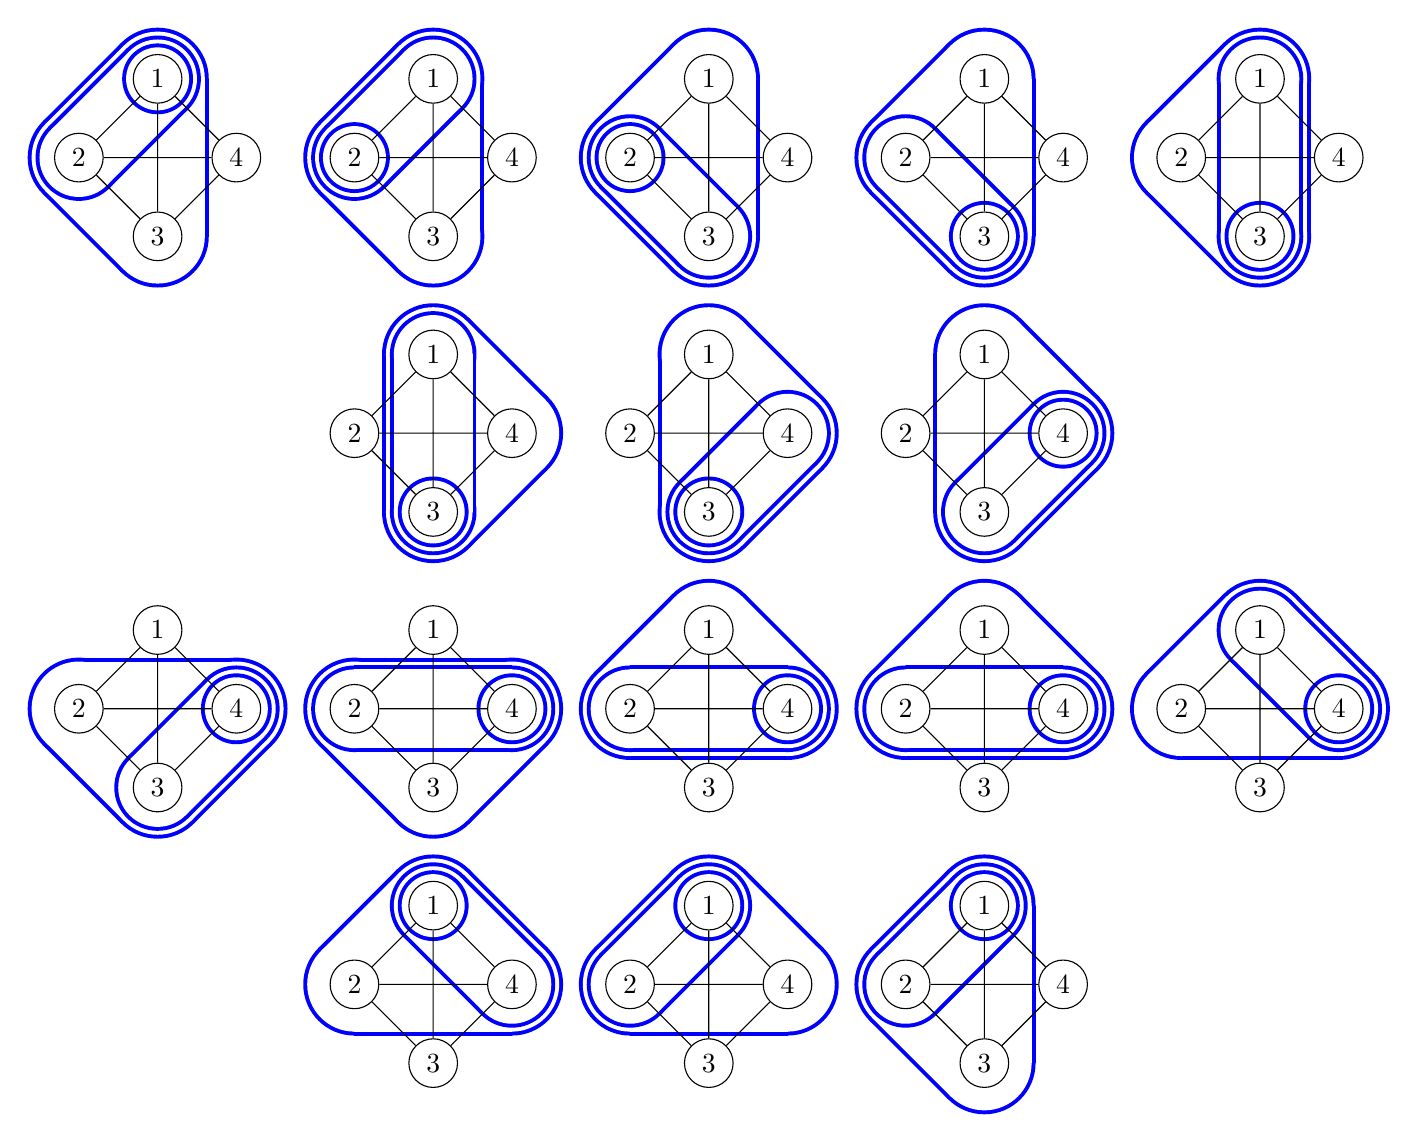
\begin{tikzpicture}
    %1234
    \begin{scope}
        \node (1) at (90:1) [circle, draw] {1};
        \node (2) at (180:1) [circle, draw] {2};
        \node (3) at (270:1) [circle, draw] {3};
        \node (4) at (0:1) [circle, draw] {4};          \draw (1) -- (2) -- (3) -- (4) -- (2) (3) -- (1) -- (4);

    
        %Tube 123
        \begin{scope}[on background layer]
            \fill[\tubecolor] (1) circle (\n + 5*\thickness);
            \fill[\tubecolor] (2) circle (\n + 5*\thickness);
            \fill[\tubecolor] (3) circle (\n + 5*\thickness);
            \draw[\tubecolor] [line width = 2*(\n + 5*\thickness)] (1.center) -- (2.center);
            \draw[\tubecolor] [line width = 2*(\n + 5*\thickness)] (2.center) -- (3.center);
            \draw[\tubecolor] [line width = 2*(\n + 5*\thickness)] (1.center) -- (3.center);
            
            \fill[white] (1) circle (\n + 4*\thickness);
            \fill[white] (2) circle (\n + 4*\thickness);
            \fill[white] (3) circle (\n + 4*\thickness);
            \draw[white] [line width = 2*(\n + 4*\thickness)] (1.center) -- (2.center);
            \draw[white] [line width = 2*(\n + 4*\thickness)] (2.center) -- (3.center);
            \draw[white] [line width = 2*(\n + 4*\thickness)] (1.center) -- (3.center);
        \end{scope}
        %Tube 12
        \begin{scope}[on background layer]
            \fill[\tubecolor] (1) circle (\n + 3*\thickness);
            \fill[\tubecolor] (2) circle (\n + 3*\thickness);
            \draw[\tubecolor] [line width = 2*(\n + 3*\thickness)] (1.center) -- (2.center);
            
            \fill[white] (1) circle (\n + 2*\thickness);
            \fill[white] (2) circle (\n + 2*\thickness);
            \draw[white] [line width = 2*(\n + 2*\thickness)] (1.center) -- (2.center);
        \end{scope}
        %Tube 1
        \begin{scope}[on background layer]
            \fill[\tubecolor] (1) circle (\n + 1*\thickness);
            
            \fill[white] (1) circle (\n + 0*\thickness);
        \end{scope}
   
    \end{scope}
    %2134
    \begin{scope}[xshift = 3.5cm]
        \node (1) at (90:1) [circle, draw] {1};
        \node (2) at (180:1) [circle, draw] {2};
        \node (3) at (270:1) [circle, draw] {3};
        \node (4) at (0:1) [circle, draw] {4};          \draw (1) -- (2) -- (3) -- (4) -- (2) (3) -- (1) -- (4);
    
        %Tube 123
        \begin{scope}[on background layer]
            \fill[\tubecolor] (1) circle (\n + 5*\thickness);
            \fill[\tubecolor] (2) circle (\n + 5*\thickness);
            \fill[\tubecolor] (3) circle (\n + 5*\thickness);
            \draw[\tubecolor] [line width = 2*(\n + 5*\thickness)] (1.center) -- (2.center);
            \draw[\tubecolor] [line width = 2*(\n + 5*\thickness)] (2.center) -- (3.center);
            \draw[\tubecolor] [line width = 2*(\n + 5*\thickness)] (1.center) -- (3.center);
            
            \fill[white] (1) circle (\n + 4*\thickness);
            \fill[white] (2) circle (\n + 4*\thickness);
            \fill[white] (3) circle (\n + 4*\thickness);
            \draw[white] [line width = 2*(\n + 4*\thickness)] (1.center) -- (2.center);
            \draw[white] [line width = 2*(\n + 4*\thickness)] (2.center) -- (3.center);
            \draw[white] [line width = 2*(\n + 4*\thickness)] (1.center) -- (3.center);
        \end{scope}
        %Tube 12
        \begin{scope}[on background layer]
            \fill[\tubecolor] (1) circle (\n + 3*\thickness);
            \fill[\tubecolor] (2) circle (\n + 3*\thickness);
            \draw[\tubecolor] [line width = 2*(\n + 3*\thickness)] (1.center) -- (2.center);
            
            \fill[white] (1) circle (\n + 2*\thickness);
            \fill[white] (2) circle (\n + 2*\thickness);
            \draw[white] [line width = 2*(\n + 2*\thickness)] (1.center) -- (2.center);
        \end{scope}
        %Tube 2
        \begin{scope}[on background layer]
            \fill[\tubecolor] (2) circle (\n + 1*\thickness);
            
            \fill[white] (2) circle (\n + 0*\thickness);
        \end{scope}
   
    \end{scope}
    %2314
    \begin{scope}[xshift = 7cm]
        \node (1) at (90:1) [circle, draw] {1};
        \node (2) at (180:1) [circle, draw] {2};
        \node (3) at (270:1) [circle, draw] {3};
        \node (4) at (0:1) [circle, draw] {4};          \draw (1) -- (2) -- (3) -- (4) -- (2) (3) -- (1) -- (4);
    
        %Tube 123
        \begin{scope}[on background layer]
            \fill[\tubecolor] (1) circle (\n + 5*\thickness);
            \fill[\tubecolor] (2) circle (\n + 5*\thickness);
            \fill[\tubecolor] (3) circle (\n + 5*\thickness);
            \draw[\tubecolor] [line width = 2*(\n + 5*\thickness)] (1.center) -- (2.center);
            \draw[\tubecolor] [line width = 2*(\n + 5*\thickness)] (2.center) -- (3.center);
            \draw[\tubecolor] [line width = 2*(\n + 5*\thickness)] (1.center) -- (3.center);
            
            \fill[white] (1) circle (\n + 4*\thickness);
            \fill[white] (2) circle (\n + 4*\thickness);
            \fill[white] (3) circle (\n + 4*\thickness);
            \draw[white] [line width = 2*(\n + 4*\thickness)] (1.center) -- (2.center);
            \draw[white] [line width = 2*(\n + 4*\thickness)] (2.center) -- (3.center);
            \draw[white] [line width = 2*(\n + 4*\thickness)] (1.center) -- (3.center);
        \end{scope}
        %Tube 23
        \begin{scope}[on background layer]
            \fill[\tubecolor] (3) circle (\n + 3*\thickness);
            \fill[\tubecolor] (2) circle (\n + 3*\thickness);
            \draw[\tubecolor] [line width = 2*(\n + 3*\thickness)] (3.center) -- (2.center);
            
            \fill[white] (3) circle (\n + 2*\thickness);
            \fill[white] (2) circle (\n + 2*\thickness);
            \draw[white] [line width = 2*(\n + 2*\thickness)] (3.center) -- (2.center);
        \end{scope}
        %Tube 2
        \begin{scope}[on background layer]
            \fill[\tubecolor] (2) circle (\n + 1*\thickness);
            
            \fill[white] (2) circle (\n + 0*\thickness);
        \end{scope}
   
    \end{scope}
    %3214
    \begin{scope}[xshift = 10.5cm]
        \node (1) at (90:1) [circle, draw] {1};
        \node (2) at (180:1) [circle, draw] {2};
        \node (3) at (270:1) [circle, draw] {3};
        \node (4) at (0:1) [circle, draw] {4};          \draw (1) -- (2) -- (3) -- (4) -- (2) (3) -- (1) -- (4);
    
        %Tube 123
        \begin{scope}[on background layer]
            \fill[\tubecolor] (1) circle (\n + 5*\thickness);
            \fill[\tubecolor] (2) circle (\n + 5*\thickness);
            \fill[\tubecolor] (3) circle (\n + 5*\thickness);
            \draw[\tubecolor] [line width = 2*(\n + 5*\thickness)] (1.center) -- (2.center);
            \draw[\tubecolor] [line width = 2*(\n + 5*\thickness)] (2.center) -- (3.center);
            \draw[\tubecolor] [line width = 2*(\n + 5*\thickness)] (1.center) -- (3.center);
            
            \fill[white] (1) circle (\n + 4*\thickness);
            \fill[white] (2) circle (\n + 4*\thickness);
            \fill[white] (3) circle (\n + 4*\thickness);
            \draw[white] [line width = 2*(\n + 4*\thickness)] (1.center) -- (2.center);
            \draw[white] [line width = 2*(\n + 4*\thickness)] (2.center) -- (3.center);
            \draw[white] [line width = 2*(\n + 4*\thickness)] (1.center) -- (3.center);
        \end{scope}
        %Tube 23
        \begin{scope}[on background layer]
            \fill[\tubecolor] (3) circle (\n + 3*\thickness);
            \fill[\tubecolor] (2) circle (\n + 3*\thickness);
            \draw[\tubecolor] [line width = 2*(\n + 3*\thickness)] (3.center) -- (2.center);
            
            \fill[white] (3) circle (\n + 2*\thickness);
            \fill[white] (2) circle (\n + 2*\thickness);
            \draw[white] [line width = 2*(\n + 2*\thickness)] (3.center) -- (2.center);
        \end{scope}
        %Tube 3
        \begin{scope}[on background layer]
            \fill[\tubecolor] (3) circle (\n + 1*\thickness);
            
            \fill[white] (3) circle (\n + 0*\thickness);
        \end{scope}
   
    \end{scope}
    %3124
    \begin{scope}[xshift = 14cm]
        \node (1) at (90:1) [circle, draw] {1};
        \node (2) at (180:1) [circle, draw] {2};
        \node (3) at (270:1) [circle, draw] {3};
        \node (4) at (0:1) [circle, draw] {4};          \draw (1) -- (2) -- (3) -- (4) -- (2) (3) -- (1) -- (4);

    
        %Tube 123
        \begin{scope}[on background layer]
            \fill[\tubecolor] (1) circle (\n + 5*\thickness);
            \fill[\tubecolor] (2) circle (\n + 5*\thickness);
            \fill[\tubecolor] (3) circle (\n + 5*\thickness);
            \draw[\tubecolor] [line width = 2*(\n + 5*\thickness)] (1.center) -- (2.center);
            \draw[\tubecolor] [line width = 2*(\n + 5*\thickness)] (2.center) -- (3.center);
            \draw[\tubecolor] [line width = 2*(\n + 5*\thickness)] (1.center) -- (3.center);
            
            \fill[white] (1) circle (\n + 4*\thickness);
            \fill[white] (2) circle (\n + 4*\thickness);
            \fill[white] (3) circle (\n + 4*\thickness);
            \draw[white] [line width = 2*(\n + 4*\thickness)] (1.center) -- (2.center);
            \draw[white] [line width = 2*(\n + 4*\thickness)] (2.center) -- (3.center);
            \draw[white] [line width = 2*(\n + 4*\thickness)] (1.center) -- (3.center);
        \end{scope}
        %Tube 13
        \begin{scope}[on background layer]
            \fill[\tubecolor] (3) circle (\n + 3*\thickness);
            \fill[\tubecolor] (1) circle (\n + 3*\thickness);
            \draw[\tubecolor] [line width = 2*(\n + 3*\thickness)] (3.center) -- (1.center);
            
            \fill[white] (3) circle (\n + 2*\thickness);
            \fill[white] (1) circle (\n + 2*\thickness);
            \draw[white] [line width = 2*(\n + 2*\thickness)] (3.center) -- (1.center);
        \end{scope}
        %Tube 3
        \begin{scope}[on background layer]
            \fill[\tubecolor] (3) circle (\n + 1*\thickness);
            
            \fill[white] (3) circle (\n + 0*\thickness);
        \end{scope}
    \end{scope}
    %3142
    \begin{scope}[xshift = 3.5cm, yshift = -3.5cm]
        
        
        \node (1) at (90:1) [circle, draw] {1};
        \node (2) at (180:1) [circle, draw] {2};
        \node (3) at (270:1) [circle, draw] {3};
        \node (4) at (0:1) [circle, draw] {4};          \draw (1) -- (2) -- (3) -- (4) -- (2) (3) -- (1) -- (4);
    
        %Tube 134
        \begin{scope}[on background layer]
            \fill[\tubecolor] (1) circle (\n + 5*\thickness);
            \fill[\tubecolor] (4) circle (\n + 5*\thickness);
            \fill[\tubecolor] (3) circle (\n + 5*\thickness);
            \draw[\tubecolor] [line width = 2*(\n + 5*\thickness)] (1.center) -- (4.center);
            \draw[\tubecolor] [line width = 2*(\n + 5*\thickness)] (4.center) -- (3.center);
            \draw[\tubecolor] [line width = 2*(\n + 5*\thickness)] (1.center) -- (3.center);
            
            \fill[white] (1) circle (\n + 4*\thickness);
            \fill[white] (4) circle (\n + 4*\thickness);
            \fill[white] (3) circle (\n + 4*\thickness);
            \draw[white] [line width = 2*(\n + 4*\thickness)] (1.center) -- (4.center);
            \draw[white] [line width = 2*(\n + 4*\thickness)] (4.center) -- (3.center);
            \draw[white] [line width = 2*(\n + 4*\thickness)] (1.center) -- (3.center);
        \end{scope}
        %Tube 13
        \begin{scope}[on background layer]
            \fill[\tubecolor] (3) circle (\n + 3*\thickness);
            \fill[\tubecolor] (1) circle (\n + 3*\thickness);
            \draw[\tubecolor] [line width = 2*(\n + 3*\thickness)] (3.center) -- (1.center);
            
            \fill[white] (3) circle (\n + 2*\thickness);
            \fill[white] (1) circle (\n + 2*\thickness);
            \draw[white] [line width = 2*(\n + 2*\thickness)] (3.center) -- (1.center);
        \end{scope}
        %Tube 3
        \begin{scope}[on background layer]
            \fill[\tubecolor] (3) circle (\n + 1*\thickness);
            
            \fill[white] (3) circle (\n + 0*\thickness);
        \end{scope}
    
    \end{scope}
    %3412
    \begin{scope}[xshift = 7cm, yshift = -3.5cm]
        \node (1) at (90:1) [circle, draw] {1};
        \node (2) at (180:1) [circle, draw] {2};
        \node (3) at (270:1) [circle, draw] {3};
        \node (4) at (0:1) [circle, draw] {4};          \draw (1) -- (2) -- (3) -- (4) -- (2) (3) -- (1) -- (4);
    
        %Tube 134
        \begin{scope}[on background layer]
            \fill[\tubecolor] (1) circle (\n + 5*\thickness);
            \fill[\tubecolor] (4) circle (\n + 5*\thickness);
            \fill[\tubecolor] (3) circle (\n + 5*\thickness);
            \draw[\tubecolor] [line width = 2*(\n + 5*\thickness)] (1.center) -- (4.center);
            \draw[\tubecolor] [line width = 2*(\n + 5*\thickness)] (4.center) -- (3.center);
            \draw[\tubecolor] [line width = 2*(\n + 5*\thickness)] (1.center) -- (3.center);
            
            \fill[white] (1) circle (\n + 4*\thickness);
            \fill[white] (4) circle (\n + 4*\thickness);
            \fill[white] (3) circle (\n + 4*\thickness);
            \draw[white] [line width = 2*(\n + 4*\thickness)] (1.center) -- (4.center);
            \draw[white] [line width = 2*(\n + 4*\thickness)] (4.center) -- (3.center);
            \draw[white] [line width = 2*(\n + 4*\thickness)] (1.center) -- (3.center);
        \end{scope}
        %Tube 34
        \begin{scope}[on background layer]
            \fill[\tubecolor] (3) circle (\n + 3*\thickness);
            \fill[\tubecolor] (4) circle (\n + 3*\thickness);
            \draw[\tubecolor] [line width = 2*(\n + 3*\thickness)] (3.center) -- (4.center);
            
            \fill[white] (3) circle (\n + 2*\thickness);
            \fill[white] (4) circle (\n + 2*\thickness);
            \draw[white] [line width = 2*(\n + 2*\thickness)] (3.center) -- (4.center);
        \end{scope}
        %Tube 3
        \begin{scope}[on background layer]
            \fill[\tubecolor] (3) circle (\n + 1*\thickness);
            
            \fill[white] (3) circle (\n + 0*\thickness);
        \end{scope}
    
    \end{scope}
    %4312
    \begin{scope}[xshift = 10.5cm, yshift = -3.5cm]
        \node (1) at (90:1) [circle, draw] {1};
        \node (2) at (180:1) [circle, draw] {2};
        \node (3) at (270:1) [circle, draw] {3};
        \node (4) at (0:1) [circle, draw] {4};          \draw (1) -- (2) -- (3) -- (4) -- (2) (3) -- (1) -- (4);
    
        %Tube 134
        \begin{scope}[on background layer]
            \fill[\tubecolor] (1) circle (\n + 5*\thickness);
            \fill[\tubecolor] (4) circle (\n + 5*\thickness);
            \fill[\tubecolor] (3) circle (\n + 5*\thickness);
            \draw[\tubecolor] [line width = 2*(\n + 5*\thickness)] (1.center) -- (4.center);
            \draw[\tubecolor] [line width = 2*(\n + 5*\thickness)] (4.center) -- (3.center);
            \draw[\tubecolor] [line width = 2*(\n + 5*\thickness)] (1.center) -- (3.center);
            
            \fill[white] (1) circle (\n + 4*\thickness);
            \fill[white] (4) circle (\n + 4*\thickness);
            \fill[white] (3) circle (\n + 4*\thickness);
            \draw[white] [line width = 2*(\n + 4*\thickness)] (1.center) -- (4.center);
            \draw[white] [line width = 2*(\n + 4*\thickness)] (4.center) -- (3.center);
            \draw[white] [line width = 2*(\n + 4*\thickness)] (1.center) -- (3.center);
        \end{scope}
        %Tube 34
        \begin{scope}[on background layer]
            \fill[\tubecolor] (3) circle (\n + 3*\thickness);
            \fill[\tubecolor] (4) circle (\n + 3*\thickness);
            \draw[\tubecolor] [line width = 2*(\n + 3*\thickness)] (3.center) -- (4.center);
            
            \fill[white] (3) circle (\n + 2*\thickness);
            \fill[white] (4) circle (\n + 2*\thickness);
            \draw[white] [line width = 2*(\n + 2*\thickness)] (3.center) -- (4.center);
        \end{scope}
        %Tube 4
        \begin{scope}[on background layer]
            \fill[\tubecolor] (4) circle (\n + 1*\thickness);
            
            \fill[white] (4) circle (\n + 0*\thickness);
        \end{scope}
    \end{scope}
    %4321
    \begin{scope}[xshift = 0cm, yshift = -7cm]
        \node (1) at (90:1) [circle, draw] {1};
        \node (2) at (180:1) [circle, draw] {2};
        \node (3) at (270:1) [circle, draw] {3};
        \node (4) at (0:1) [circle, draw] {4};          \draw (1) -- (2) -- (3) -- (4) -- (2) (3) -- (1) -- (4);
    
        %Tube 234
        \begin{scope}[on background layer]
            \fill[\tubecolor] (2) circle (\n + 5*\thickness);
            \fill[\tubecolor] (4) circle (\n + 5*\thickness);
            \fill[\tubecolor] (3) circle (\n + 5*\thickness);
            \draw[\tubecolor] [line width = 2*(\n + 5*\thickness)] (2.center) -- (4.center);
            \draw[\tubecolor] [line width = 2*(\n + 5*\thickness)] (4.center) -- (3.center);
            \draw[\tubecolor] [line width = 2*(\n + 5*\thickness)] (2.center) -- (3.center);
            
            \fill[white] (2) circle (\n + 4*\thickness);
            \fill[white] (4) circle (\n + 4*\thickness);
            \fill[white] (3) circle (\n + 4*\thickness);
            \draw[white] [line width = 2*(\n + 4*\thickness)] (2.center) -- (4.center);
            \draw[white] [line width = 2*(\n + 4*\thickness)] (4.center) -- (3.center);
            \draw[white] [line width = 2*(\n + 4*\thickness)] (2.center) -- (3.center);
        \end{scope}
        %Tube 34
        \begin{scope}[on background layer]
            \fill[\tubecolor] (3) circle (\n + 3*\thickness);
            \fill[\tubecolor] (4) circle (\n + 3*\thickness);
            \draw[\tubecolor] [line width = 2*(\n + 3*\thickness)] (3.center) -- (4.center);
            
            \fill[white] (3) circle (\n + 2*\thickness);
            \fill[white] (4) circle (\n + 2*\thickness);
            \draw[white] [line width = 2*(\n + 2*\thickness)] (3.center) -- (4.center);
        \end{scope}
        %Tube 4
        \begin{scope}[on background layer]
            \fill[\tubecolor] (4) circle (\n + 1*\thickness);
            
            \fill[white] (4) circle (\n + 0*\thickness);
        \end{scope}
        
    \end{scope}
    %4231
    \begin{scope}[xshift = 3.5cm, yshift = -7cm]
        \node (1) at (90:1) [circle, draw] {1};
        \node (2) at (180:1) [circle, draw] {2};
        \node (3) at (270:1) [circle, draw] {3};
        \node (4) at (0:1) [circle, draw] {4};          \draw (1) -- (2) -- (3) -- (4) -- (2) (3) -- (1) -- (4);
    
        %Tube 234
        \begin{scope}[on background layer]
            \fill[\tubecolor] (2) circle (\n + 5*\thickness);
            \fill[\tubecolor] (4) circle (\n + 5*\thickness);
            \fill[\tubecolor] (3) circle (\n + 5*\thickness);
            \draw[\tubecolor] [line width = 2*(\n + 5*\thickness)] (2.center) -- (4.center);
            \draw[\tubecolor] [line width = 2*(\n + 5*\thickness)] (4.center) -- (3.center);
            \draw[\tubecolor] [line width = 2*(\n + 5*\thickness)] (2.center) -- (3.center);
            
            \fill[white] (2) circle (\n + 4*\thickness);
            \fill[white] (4) circle (\n + 4*\thickness);
            \fill[white] (3) circle (\n + 4*\thickness);
            \draw[white] [line width = 2*(\n + 4*\thickness)] (2.center) -- (4.center);
            \draw[white] [line width = 2*(\n + 4*\thickness)] (4.center) -- (3.center);
            \draw[white] [line width = 2*(\n + 4*\thickness)] (2.center) -- (3.center);
        \end{scope}
        %Tube 24
        \begin{scope}[on background layer]
            \fill[\tubecolor] (2) circle (\n + 3*\thickness);
            \fill[\tubecolor] (4) circle (\n + 3*\thickness);
            \draw[\tubecolor] [line width = 2*(\n + 3*\thickness)] (2.center) -- (4.center);
            
            \fill[white] (2) circle (\n + 2*\thickness);
            \fill[white] (4) circle (\n + 2*\thickness);
            \draw[white] [line width = 2*(\n + 2*\thickness)] (2.center) -- (4.center);
        \end{scope}
        %Tube 4
        \begin{scope}[on background layer]
            \fill[\tubecolor] (4) circle (\n + 1*\thickness);
            
            \fill[white] (4) circle (\n + 0*\thickness);
        \end{scope}
        
    \end{scope}
    %4213
    \begin{scope}[xshift = 7cm, yshift = -7cm]
        \node (1) at (90:1) [circle, draw] {1};
        \node (2) at (180:1) [circle, draw] {2};
        \node (3) at (270:1) [circle, draw] {3};
        \node (4) at (0:1) [circle, draw] {4};          \draw (1) -- (2) -- (3) -- (4) -- (2) (3) -- (1) -- (4);
    
        %Tube 124
        \begin{scope}[on background layer]
            \fill[\tubecolor] (2) circle (\n + 5*\thickness);
            \fill[\tubecolor] (4) circle (\n + 5*\thickness);
            \fill[\tubecolor] (1) circle (\n + 5*\thickness);
            \draw[\tubecolor] [line width = 2*(\n + 5*\thickness)] (2.center) -- (4.center);
            \draw[\tubecolor] [line width = 2*(\n + 5*\thickness)] (4.center) -- (1.center);
            \draw[\tubecolor] [line width = 2*(\n + 5*\thickness)] (2.center) -- (1.center);
            
            \fill[white] (2) circle (\n + 4*\thickness);
            \fill[white] (4) circle (\n + 4*\thickness);
            \fill[white] (1) circle (\n + 4*\thickness);
            \draw[white] [line width = 2*(\n + 4*\thickness)] (2.center) -- (4.center);
            \draw[white] [line width = 2*(\n + 4*\thickness)] (4.center) -- (1.center);
            \draw[white] [line width = 2*(\n + 4*\thickness)] (2.center) -- (1.center);
        \end{scope}
        %Tube 24
        \begin{scope}[on background layer]
            \fill[\tubecolor] (2) circle (\n + 3*\thickness);
            \fill[\tubecolor] (4) circle (\n + 3*\thickness);
            \draw[\tubecolor] [line width = 2*(\n + 3*\thickness)] (2.center) -- (4.center);
            
            \fill[white] (2) circle (\n + 2*\thickness);
            \fill[white] (4) circle (\n + 2*\thickness);
            \draw[white] [line width = 2*(\n + 2*\thickness)] (2.center) -- (4.center);
        \end{scope}
        %Tube 4
        \begin{scope}[on background layer]
            \fill[\tubecolor] (4) circle (\n + 1*\thickness);
            
            \fill[white] (4) circle (\n + 0*\thickness);
        \end{scope}
        
    \end{scope}
    %4213
    \begin{scope}[xshift = 10.5cm, yshift = -7cm]
        \node (1) at (90:1) [circle, draw] {1};
        \node (2) at (180:1) [circle, draw] {2};
        \node (3) at (270:1) [circle, draw] {3};
        \node (4) at (0:1) [circle, draw] {4};          \draw (1) -- (2) -- (3) -- (4) -- (2) (3) -- (1) -- (4);
    
        %Tube 124
        \begin{scope}[on background layer]
            \fill[\tubecolor] (2) circle (\n + 5*\thickness);
            \fill[\tubecolor] (4) circle (\n + 5*\thickness);
            \fill[\tubecolor] (1) circle (\n + 5*\thickness);
            \draw[\tubecolor] [line width = 2*(\n + 5*\thickness)] (2.center) -- (4.center);
            \draw[\tubecolor] [line width = 2*(\n + 5*\thickness)] (4.center) -- (1.center);
            \draw[\tubecolor] [line width = 2*(\n + 5*\thickness)] (2.center) -- (1.center);
            
            \fill[white] (2) circle (\n + 4*\thickness);
            \fill[white] (4) circle (\n + 4*\thickness);
            \fill[white] (1) circle (\n + 4*\thickness);
            \draw[white] [line width = 2*(\n + 4*\thickness)] (2.center) -- (4.center);
            \draw[white] [line width = 2*(\n + 4*\thickness)] (4.center) -- (1.center);
            \draw[white] [line width = 2*(\n + 4*\thickness)] (2.center) -- (1.center);
        \end{scope}
        %Tube 24
        \begin{scope}[on background layer]
            \fill[\tubecolor] (2) circle (\n + 3*\thickness);
            \fill[\tubecolor] (4) circle (\n + 3*\thickness);
            \draw[\tubecolor] [line width = 2*(\n + 3*\thickness)] (2.center) -- (4.center);
            
            \fill[white] (2) circle (\n + 2*\thickness);
            \fill[white] (4) circle (\n + 2*\thickness);
            \draw[white] [line width = 2*(\n + 2*\thickness)] (2.center) -- (4.center);
        \end{scope}
        %Tube 4
        \begin{scope}[on background layer]
            \fill[\tubecolor] (4) circle (\n + 1*\thickness);
            
            \fill[white] (4) circle (\n + 0*\thickness);
        \end{scope}
        
    \end{scope}
    %4123
    \begin{scope}[xshift = 14cm, yshift = -7cm]
        \node (1) at (90:1) [circle, draw] {1};
        \node (2) at (180:1) [circle, draw] {2};
        \node (3) at (270:1) [circle, draw] {3};
        \node (4) at (0:1) [circle, draw] {4};          \draw (1) -- (2) -- (3) -- (4) -- (2) (3) -- (1) -- (4);
    
        %Tube 124
        \begin{scope}[on background layer]
            \fill[\tubecolor] (2) circle (\n + 5*\thickness);
            \fill[\tubecolor] (4) circle (\n + 5*\thickness);
            \fill[\tubecolor] (1) circle (\n + 5*\thickness);
            \draw[\tubecolor] [line width = 2*(\n + 5*\thickness)] (2.center) -- (4.center);
            \draw[\tubecolor] [line width = 2*(\n + 5*\thickness)] (4.center) -- (1.center);
            \draw[\tubecolor] [line width = 2*(\n + 5*\thickness)] (2.center) -- (1.center);
            
            \fill[white] (2) circle (\n + 4*\thickness);
            \fill[white] (4) circle (\n + 4*\thickness);
            \fill[white] (1) circle (\n + 4*\thickness);
            \draw[white] [line width = 2*(\n + 4*\thickness)] (2.center) -- (4.center);
            \draw[white] [line width = 2*(\n + 4*\thickness)] (4.center) -- (1.center);
            \draw[white] [line width = 2*(\n + 4*\thickness)] (2.center) -- (1.center);
        \end{scope}
        %Tube 14
        \begin{scope}[on background layer]
            \fill[\tubecolor] (1) circle (\n + 3*\thickness);
            \fill[\tubecolor] (4) circle (\n + 3*\thickness);
            \draw[\tubecolor] [line width = 2*(\n + 3*\thickness)] (1.center) -- (4.center);
            
            \fill[white] (1) circle (\n + 2*\thickness);
            \fill[white] (4) circle (\n + 2*\thickness);
            \draw[white] [line width = 2*(\n + 2*\thickness)] (1.center) -- (4.center);
        \end{scope}
        %Tube 4
        \begin{scope}[on background layer]
            \fill[\tubecolor] (4) circle (\n + 1*\thickness);
            
            \fill[white] (4) circle (\n + 0*\thickness);
        \end{scope}
    \end{scope}
    %1423
    \begin{scope}[xshift = 3.5cm, yshift = -10.5cm]
        
    
        \node (1) at (90:1) [circle, draw] {1};
        \node (2) at (180:1) [circle, draw] {2};
        \node (3) at (270:1) [circle, draw] {3};
        \node (4) at (0:1) [circle, draw] {4};          \draw (1) -- (2) -- (3) -- (4) -- (2) (3) -- (1) -- (4);
    
        %Tube 124
        \begin{scope}[on background layer]
            \fill[\tubecolor] (2) circle (\n + 5*\thickness);
            \fill[\tubecolor] (4) circle (\n + 5*\thickness);
            \fill[\tubecolor] (1) circle (\n + 5*\thickness);
            \draw[\tubecolor] [line width = 2*(\n + 5*\thickness)] (2.center) -- (4.center);
            \draw[\tubecolor] [line width = 2*(\n + 5*\thickness)] (4.center) -- (1.center);
            \draw[\tubecolor] [line width = 2*(\n + 5*\thickness)] (2.center) -- (1.center);
            
            \fill[white] (2) circle (\n + 4*\thickness);
            \fill[white] (4) circle (\n + 4*\thickness);
            \fill[white] (1) circle (\n + 4*\thickness);
            \draw[white] [line width = 2*(\n + 4*\thickness)] (2.center) -- (4.center);
            \draw[white] [line width = 2*(\n + 4*\thickness)] (4.center) -- (1.center);
            \draw[white] [line width = 2*(\n + 4*\thickness)] (2.center) -- (1.center);
        \end{scope}
        %Tube 14
        \begin{scope}[on background layer]
            \fill[\tubecolor] (1) circle (\n + 3*\thickness);
            \fill[\tubecolor] (4) circle (\n + 3*\thickness);
            \draw[\tubecolor] [line width = 2*(\n + 3*\thickness)] (1.center) -- (4.center);
            
            \fill[white] (1) circle (\n + 2*\thickness);
            \fill[white] (4) circle (\n + 2*\thickness);
            \draw[white] [line width = 2*(\n + 2*\thickness)] (1.center) -- (4.center);
        \end{scope}
        %Tube 1
        \begin{scope}[on background layer]
            \fill[\tubecolor] (1) circle (\n + 1*\thickness);
            
            \fill[white] (1) circle (\n + 0*\thickness);
        \end{scope}
        
    \end{scope}
    %1243
    \begin{scope}[xshift = 7cm, yshift = -10.5cm]
        \node (1) at (90:1) [circle, draw] {1};
        \node (2) at (180:1) [circle, draw] {2};
        \node (3) at (270:1) [circle, draw] {3};
        \node (4) at (0:1) [circle, draw] {4};          \draw (1) -- (2) -- (3) -- (4) -- (2) (3) -- (1) -- (4);
    
        %Tube 124
        \begin{scope}[on background layer]
            \fill[\tubecolor] (2) circle (\n + 5*\thickness);
            \fill[\tubecolor] (4) circle (\n + 5*\thickness);
            \fill[\tubecolor] (1) circle (\n + 5*\thickness);
            \draw[\tubecolor] [line width = 2*(\n + 5*\thickness)] (2.center) -- (4.center);
            \draw[\tubecolor] [line width = 2*(\n + 5*\thickness)] (4.center) -- (1.center);
            \draw[\tubecolor] [line width = 2*(\n + 5*\thickness)] (2.center) -- (1.center);
            
            \fill[white] (2) circle (\n + 4*\thickness);
            \fill[white] (4) circle (\n + 4*\thickness);
            \fill[white] (1) circle (\n + 4*\thickness);
            \draw[white] [line width = 2*(\n + 4*\thickness)] (2.center) -- (4.center);
            \draw[white] [line width = 2*(\n + 4*\thickness)] (4.center) -- (1.center);
            \draw[white] [line width = 2*(\n + 4*\thickness)] (2.center) -- (1.center);
        \end{scope}
        %Tube 12
        \begin{scope}[on background layer]
            \fill[\tubecolor] (1) circle (\n + 3*\thickness);
            \fill[\tubecolor] (2) circle (\n + 3*\thickness);
            \draw[\tubecolor] [line width = 2*(\n + 3*\thickness)] (1.center) -- (2.center);
            
            \fill[white] (1) circle (\n + 2*\thickness);
            \fill[white] (2) circle (\n + 2*\thickness);
            \draw[white] [line width = 2*(\n + 2*\thickness)] (1.center) -- (2.center);
        \end{scope}
        %Tube 1
        \begin{scope}[on background layer]
            \fill[\tubecolor] (1) circle (\n + 1*\thickness);
            
            \fill[white] (1) circle (\n + 0*\thickness);
        \end{scope}
        
    \end{scope}
    %1234
    \begin{scope}[xshift = 10.5cm, yshift = -10.5cm]
        \node (1) at (90:1) [circle, draw] {1};
        \node (2) at (180:1) [circle, draw] {2};
        \node (3) at (270:1) [circle, draw] {3};
        \node (4) at (0:1) [circle, draw] {4};          \draw (1) -- (2) -- (3) -- (4) -- (2) (3) -- (1) -- (4);
    
        %Tube 123
        \begin{scope}[on background layer]
            \fill[\tubecolor] (2) circle (\n + 5*\thickness);
            \fill[\tubecolor] (3) circle (\n + 5*\thickness);
            \fill[\tubecolor] (1) circle (\n + 5*\thickness);
            \draw[\tubecolor] [line width = 2*(\n + 5*\thickness)] (2.center) -- (3.center);
            \draw[\tubecolor] [line width = 2*(\n + 5*\thickness)] (3.center) -- (1.center);
            \draw[\tubecolor] [line width = 2*(\n + 5*\thickness)] (2.center) -- (1.center);
            
            \fill[white] (2) circle (\n + 4*\thickness);
            \fill[white] (3) circle (\n + 4*\thickness);
            \fill[white] (1) circle (\n + 4*\thickness);
            \draw[white] [line width = 2*(\n + 4*\thickness)] (2.center) -- (3.center);
            \draw[white] [line width = 2*(\n + 4*\thickness)] (3.center) -- (1.center);
            \draw[white] [line width = 2*(\n + 4*\thickness)] (2.center) -- (1.center);
        \end{scope}
        %Tube 12
        \begin{scope}[on background layer]
            \fill[\tubecolor] (1) circle (\n + 3*\thickness);
            \fill[\tubecolor] (2) circle (\n + 3*\thickness);
            \draw[\tubecolor] [line width = 2*(\n + 3*\thickness)] (1.center) -- (2.center);
            
            \fill[white] (1) circle (\n + 2*\thickness);
            \fill[white] (2) circle (\n + 2*\thickness);
            \draw[white] [line width = 2*(\n + 2*\thickness)] (1.center) -- (2.center);
        \end{scope}
        %Tube 1
        \begin{scope}[on background layer]
            \fill[\tubecolor] (1) circle (\n + 1*\thickness);
            
            \fill[white] (1) circle (\n + 0*\thickness);
        \end{scope}
    \end{scope}
    \end{tikzpicture}
\end{center}
\end{document}